\section{memdep\_\-oracle\_\-t Class Reference}
\label{classmemdep__oracle__t}\index{memdep\_\-oracle\_\-t@{memdep\_\-oracle\_\-t}}
Inheritance diagram for memdep\_\-oracle\_\-t:\nopagebreak
\begin{figure}[H]
\begin{center}
\leavevmode
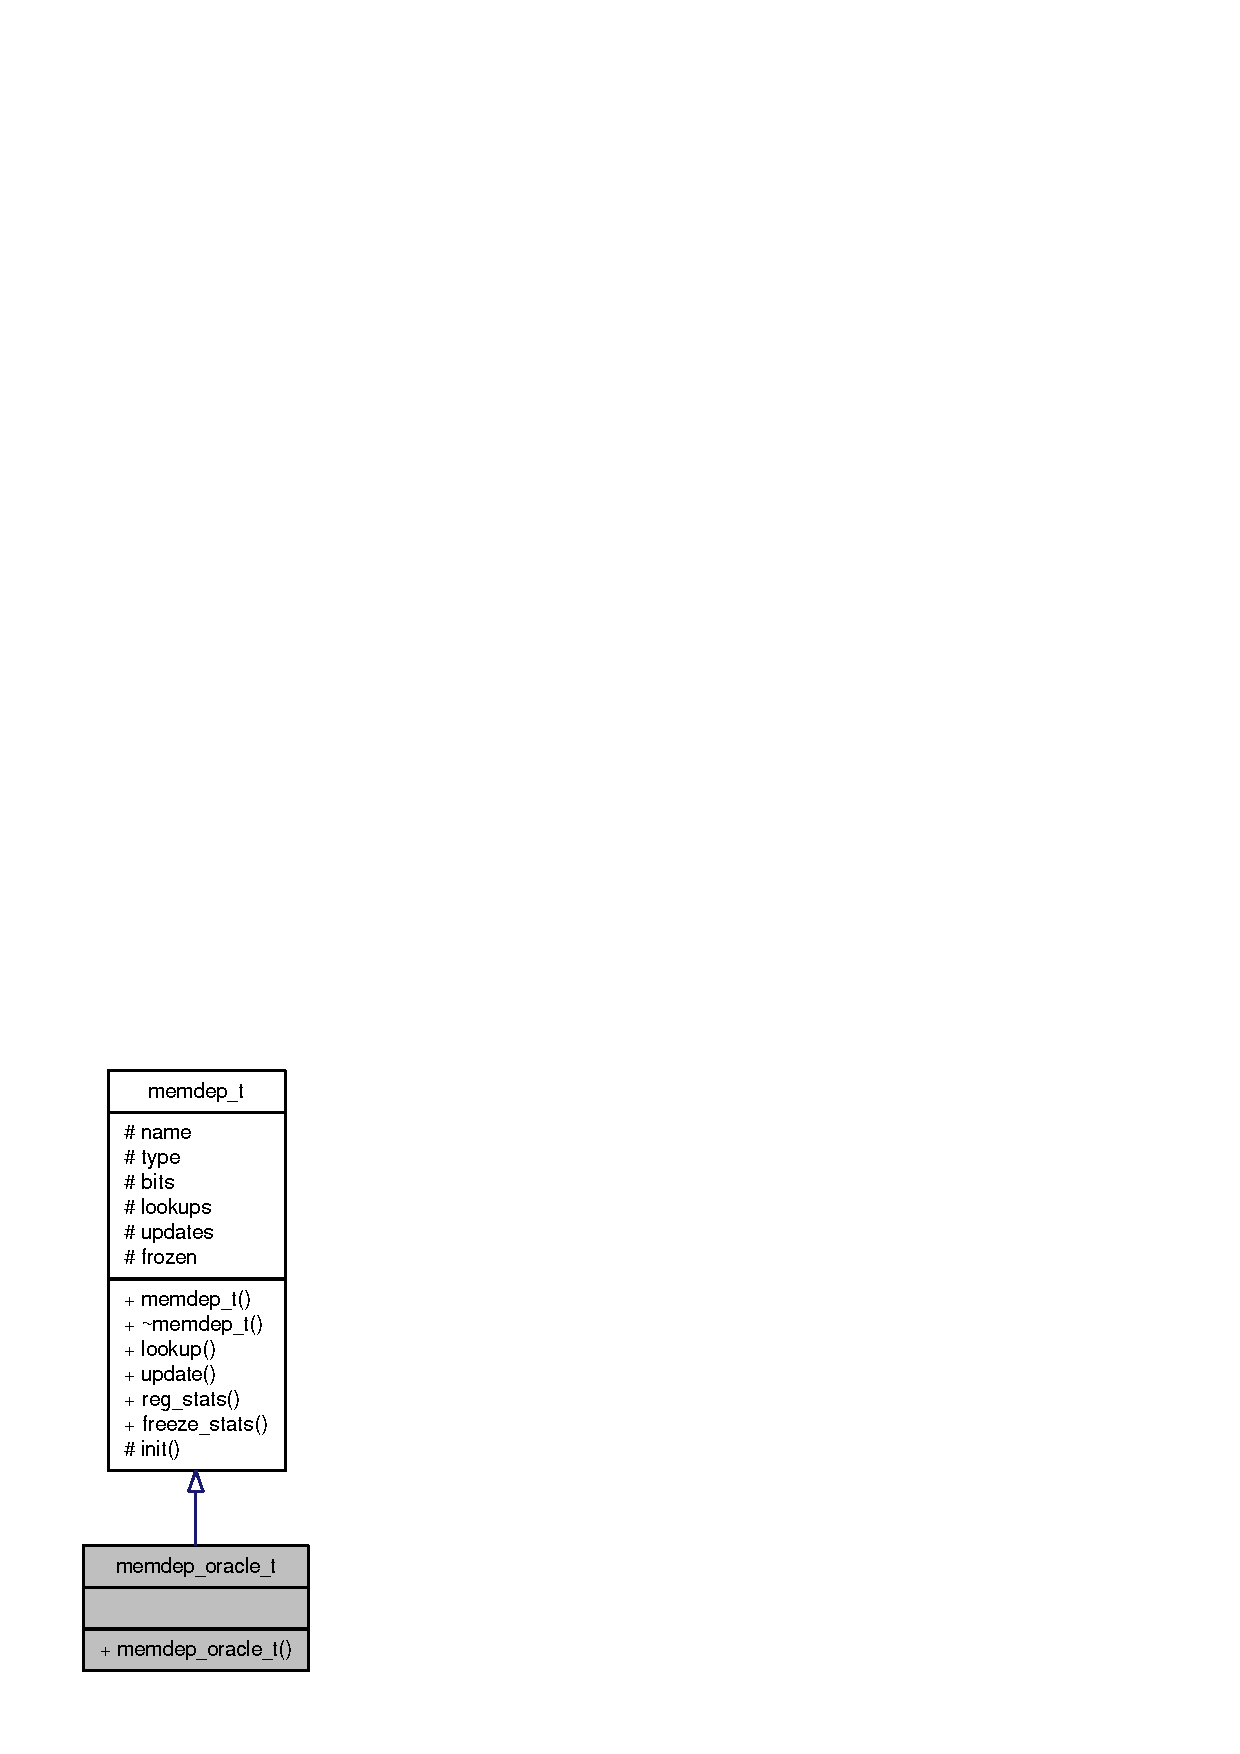
\includegraphics[width=152pt]{classmemdep__oracle__t__inherit__graph}
\end{center}
\end{figure}
Collaboration diagram for memdep\_\-oracle\_\-t:\nopagebreak
\begin{figure}[H]
\begin{center}
\leavevmode
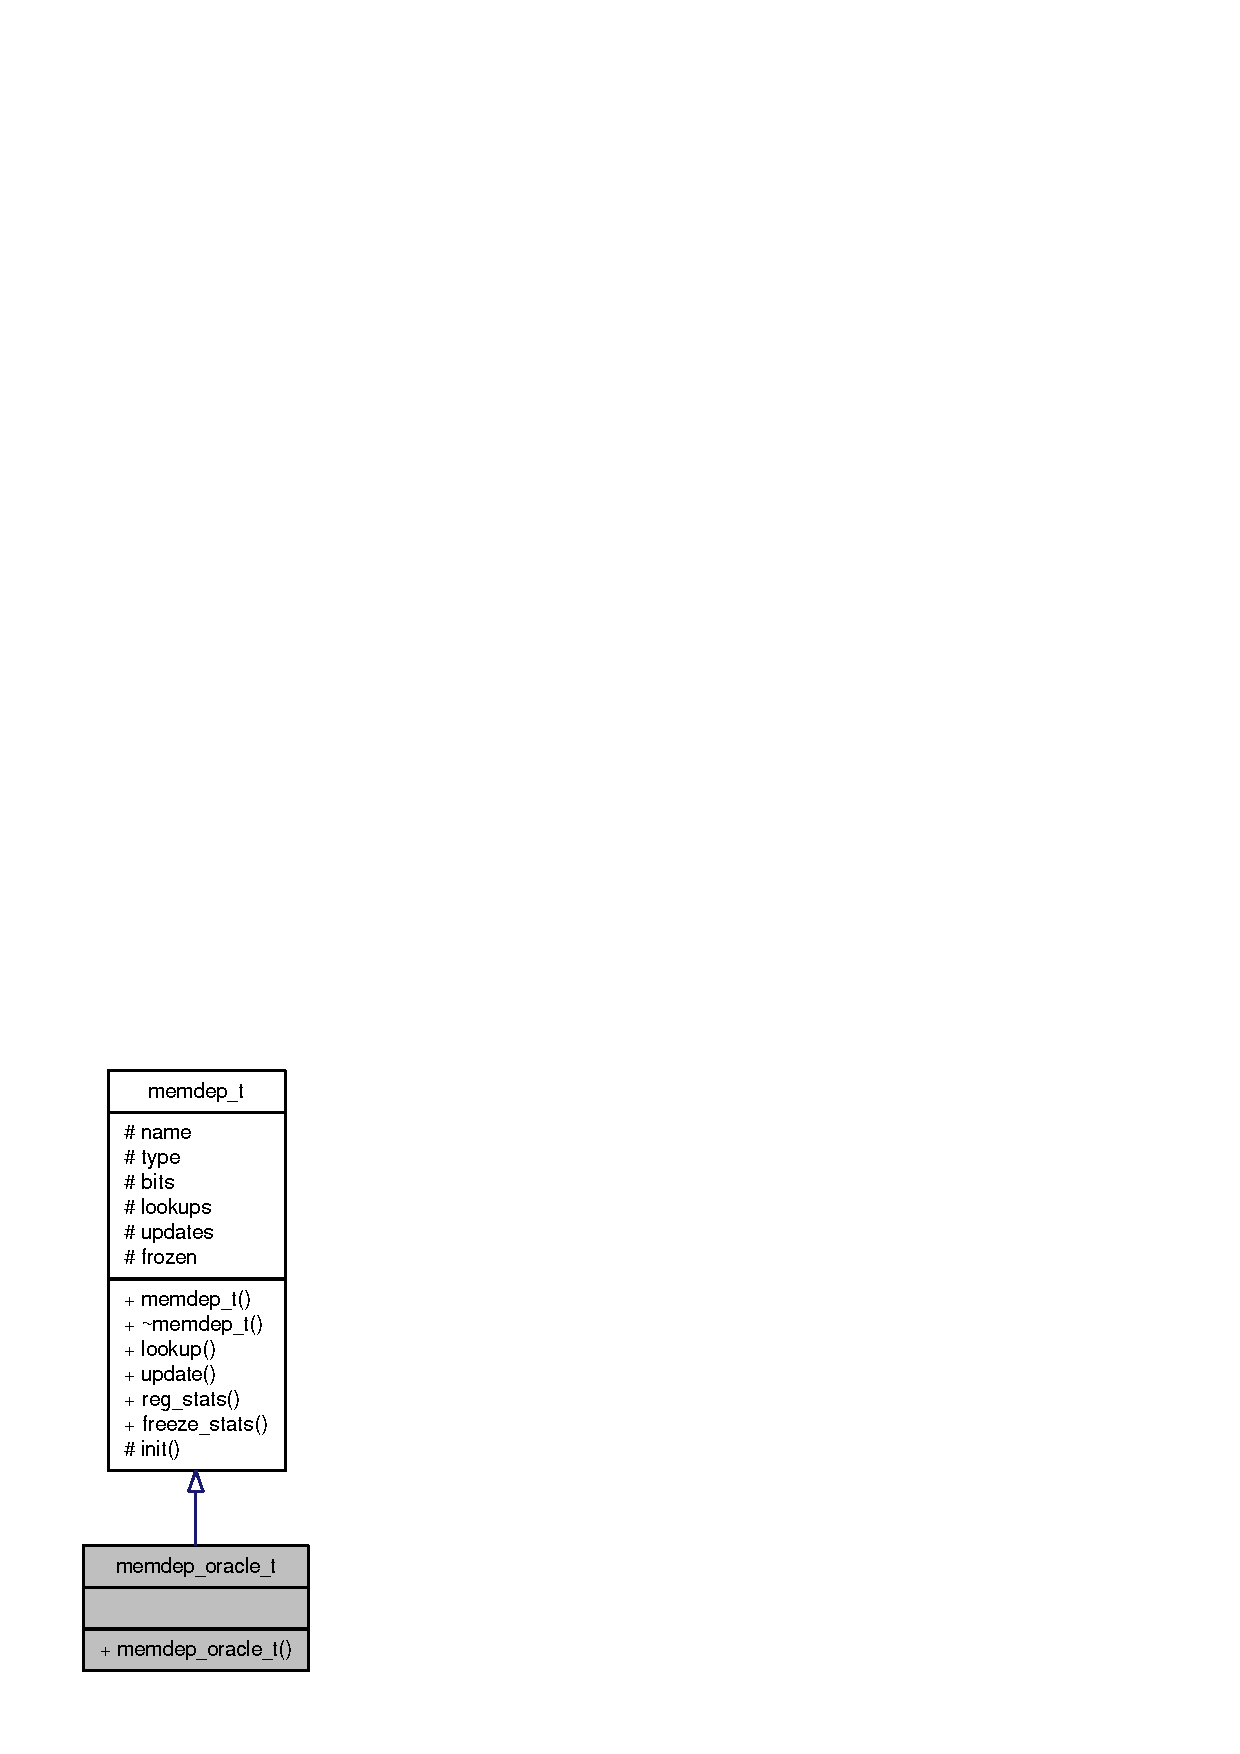
\includegraphics[width=152pt]{classmemdep__oracle__t__coll__graph}
\end{center}
\end{figure}
\subsection*{Public Member Functions}
\begin{CompactItemize}
\item 
{\bf memdep\_\-oracle\_\-t} (void)
\end{CompactItemize}


\subsection{Detailed Description}


Definition at line 16 of file memdep-oracle.cpp.

\subsection{Constructor \& Destructor Documentation}
\index{memdep\_\-oracle\_\-t@{memdep\_\-oracle\_\-t}!memdep\_\-oracle\_\-t@{memdep\_\-oracle\_\-t}}
\index{memdep\_\-oracle\_\-t@{memdep\_\-oracle\_\-t}!memdep_oracle_t@{memdep\_\-oracle\_\-t}}
\subsubsection[{memdep\_\-oracle\_\-t}]{\setlength{\rightskip}{0pt plus 5cm}memdep\_\-oracle\_\-t::memdep\_\-oracle\_\-t (void)\hspace{0.3cm}{\tt  [inline]}}\label{classmemdep__oracle__t_5ee3528e42a712d07e1af89fa5974223}




Definition at line 20 of file memdep-oracle.cpp.

References COMPONENT\_\-NAME, fatal(), memdep\_\-t::init(), memdep\_\-t::name, and memdep\_\-t::type.

The documentation for this class was generated from the following file:\begin{CompactItemize}
\item 
{\bf memdep-oracle.cpp}\end{CompactItemize}
